% Note that the a4paper option is mainly intended so that authors in
% countries using A4 can easily print to A4 and see how their papers will
% look in print - the typesetting of the document will not typically be
% affected with changes in paper size (but the bottom and side margins will).
% Use the testflow package mentioned above to verify correct handling of
% both paper sizes by the user's LaTeX system.
%
% Also note that the "draftcls" or "draftclsnofoot", not "draft", option
% should be used if it is desired that the figures are to be displayed in
% draft mode.
%
\documentclass[conference, letterpaper]{IEEEtran}
\usepackage{booktabs}
\usepackage{graphicx, tikz}
% Add the compsoc option for Computer Society conferences.
%
% If IEEEtran.cls has not been installed into the LaTeX system files,
% manually specify the path to it like:
% \documentclass[conference]{../sty/IEEEtran}


% *** MISC UTILITY PACKAGES ***
%
%\usepackage{ifpdf}
% Heiko Oberdiek's ifpdf.sty is very useful if you need conditional
% compilation based on whether the output is pdf or dvi.
% usage:
% \ifpdf
%   % pdf code
% \else
%   % dvi code
% \fi
% The latest version of ifpdf.sty can be obtained from:
% http://www.ctan.org/tex-archive/macros/latex/contrib/oberdiek/
% Also, note that IEEEtran.cls V1.7 and later provides a builtin
% \ifCLASSINFOpdf conditional that works the same way.
% When switching from latex to pdflatex and vice-versa, the compiler may
% have to be run twice to clear warning/error messages.






% *** CITATION PACKAGES ***
%
%\usepackage{cite}
% cite.sty was written by Donald Arseneau
% V1.6 and later of IEEEtran pre-defines the format of the cite.sty package
% \cite{} output to follow that of IEEE. Loading the cite package will
% result in citation numbers being automatically sorted and properly
% "compressed/ranged". e.g., [1], [9], [2], [7], [5], [6] without using
% cite.sty will become [1], [2], [5]--[7], [9] using cite.sty. cite.sty's
% \cite will automatically add leading space, if needed. Use cite.sty's
% noadjust option (cite.sty V3.8 and later) if you want to turn this off.
% cite.sty is already installed on most LaTeX systems. Be sure and use
% version 4.0 (2003-05-27) and later if using hyperref.sty. cite.sty does
% not currently provide for hyperlinked citations.
% The latest version can be obtained at:
% http://www.ctan.org/tex-archive/macros/latex/contrib/cite/
% The documentation is contained in the cite.sty file itself.




% *** GRAPHICS RELATED PACKAGES ***
%
\ifCLASSINFOpdf
  % \usepackage[pdftex]{graphicx}
  % declare the path(s) where your graphic files are
  % \graphicspath{{../pdf/}{../jpeg/}}
  % and their extensions so you won't have to specify these with
  % every instance of \includegraphics
  % \DeclareGraphicsExtensions{.pdf,.jpeg,.png}
\else
  % or other class option (dvipsone, dvipdf, if not using dvips). graphicx
  % will default to the driver specified in the system graphics.cfg if no
  % driver is specified.
  % \usepackage[dvips]{graphicx}
  % declare the path(s) where your graphic files are
  % \graphicspath{{../eps/}}
  % and their extensions so you won't have to specify these with
  % every instance of \includegraphics
  % \DeclareGraphicsExtensions{.eps}
\fi
% graphicx was written by David Carlisle and Sebastian Rahtz. It is
% required if you want graphics, photos, etc. graphicx.sty is already
% installed on most LaTeX systems. The latest version and documentation can
% be obtained at: 
% http://www.ctan.org/tex-archive/macros/latex/required/graphics/
% Another good source of documentation is "Using Imported Graphics in
% LaTeX2e" by Keith Reckdahl which can be found as epslatex.ps or
% epslatex.pdf at: http://www.ctan.org/tex-archive/info/
%
% latex, and pdflatex in dvi mode, support graphics in encapsulated
% postscript (.eps) format. pdflatex in pdf mode supports graphics
% in .pdf, .jpeg, .png and .mps (metapost) formats. Users should ensure
% that all non-photo figures use a vector format (.eps, .pdf, .mps) and
% not a bitmapped formats (.jpeg, .png). IEEE frowns on bitmapped formats
% which can result in "jaggedy"/blurry rendering of lines and letters as
% well as large increases in file sizes.
%
% You can find documentation about the pdfTeX application at:
% http://www.tug.org/applications/pdftex





\usepackage[cmex10]{amsmath}
% Also, note that the amsmath package sets \interdisplaylinepenalty to 10000
% thus preventing page breaks from occurring within multiline equations. Use:
%\interdisplaylinepenalty=2500
% after loading amsmath to restore such page breaks as IEEEtran.cls normally
% does. amsmath.sty is already installed on most LaTeX systems. The latest


% *** SPECIALIZED LIST PACKAGES ***
%
%\usepackage{algorithmic}
% algorithmic.sty was written by Peter Williams and Rogerio Brito.
% This package provides an algorithmic environment fo describing algorithms.
% You can use the algorithmic environment in-text or within a figure
% environment to provide for a floating algorithm. Do NOT use the algorithm
% floating environment provided by algorithm.sty (by the same authors) or
% algorithm2e.sty (by Christophe Fiorio) as IEEE does not use dedicated
% algorithm float types and packages that provide these will not provide
% correct IEEE style captions. The latest version and documentation of
% algorithmic.sty can be obtained at:
% http://www.ctan.org/tex-archive/macros/latex/contrib/algorithms/
% There is also a support site at:
% http://algorithms.berlios.de/index.html
% Also of interest may be the (relatively newer and more customizable)
% algorithmicx.sty package by Szasz Janos:
% http://www.ctan.org/tex-archive/macros/latex/contrib/algorithmicx/




% *** ALIGNMENT PACKAGES ***
%
%\usepackage{array}
% Frank Mittelbach's and David Carlisle's array.sty patches and improves
% the standard LaTeX2e array and tabular environments to provide better
% appearance and additional user controls. As the default LaTeX2e table
% generation code is lacking to the point of almost being broken with
% respect to the quality of the end results, all users are strongly
% advised to use an enhanced (at the very least that provided by array.sty)
% set of table tools. array.sty is already installed on most systems. The
% latest version and documentation can be obtained at:
% http://www.ctan.org/tex-archive/macros/latex/required/tools/



%\usepackage{eqparbox}
% Also of notable interest is Scott Pakin's eqparbox package for creating
% (automatically sized) equal width boxes - aka "natural width parboxes".
% Available at:
% http://www.ctan.org/tex-archive/macros/latex/contrib/eqparbox/





% *** SUBFIGURE PACKAGES ***
%\usepackage[tight,footnotesize]{subfigure}

%\usepackage[caption=false]{caption}
%\usepackage[font=footnotesize]{subfig}
% subfig.sty, also written by Steven Douglas Cochran, is the modern
% replacement for subfigure.sty. However, subfig.sty requires and
% automatically loads Axel Sommerfeldt's caption.sty which will override
% IEEEtran.cls handling of captions and this will result in nonIEEE style
% figure/table captions. To prevent this problem, be sure and preload
% caption.sty with its "caption=false" package option. This is will preserve
% IEEEtran.cls handing of captions. Version 1.3 (2005/06/28) and later 
% (recommended due to many improvements over 1.2) of subfig.sty supports
% the caption=false option directly:
%\usepackage[caption=false,font=footnotesize]{subfig}
%

% *** FLOAT PACKAGES ***
%
%\usepackage{fixltx2e}
% fixltx2e, the successor to the earlier fix2col.sty, was written by
% Frank Mittelbach and David Carlisle. This package corrects a few problems
% in the LaTeX2e kernel, the most notable of which is that in current
% LaTeX2e releases, the ordering of single and double column floats is not
% guaranteed to be preserved. Thus, an unpatched LaTeX2e can allow a
% single column figure to be placed prior to an earlier double column
% figure. The latest version and documentation can be found at:
% http://www.ctan.org/tex-archive/macros/latex/base/



%\usepackage{stfloats}
% stfloats.sty was written by Sigitas Tolusis. This package gives LaTeX2e
% the ability to do double column floats at the bottom of the page as well
% as the top. (e.g., "\begin{figure*}[!b]" is not normally possible in
% LaTeX2e). It also provides a command:
%\fnbelowfloat
% to enable the placement of footnotes below bottom floats (the standard
% LaTeX2e kernel puts them above bottom floats). This is an invasive package
% which rewrites many portions of the LaTeX2e float routines. It may not work
% with other packages that modify the LaTeX2e float routines. The latest
% version and documentation can be obtained at:
% http://www.ctan.org/tex-archive/macros/latex/contrib/sttools/
% Documentation is contained in the stfloats.sty comments as well as in the
% presfull.pdf file. Do not use the stfloats baselinefloat ability as IEEE
% does not allow \baselineskip to stretch. Authors submitting work to the
% IEEE should note that IEEE rarely uses double column equations and
% that authors should try to avoid such use. Do not be tempted to use the
% cuted.sty or midfloat.sty packages (also by Sigitas Tolusis) as IEEE does
% not format its papers in such ways.





% *** PDF, URL AND HYPERLINK PACKAGES ***
%
%\usepackage{url}
% url.sty was written by Donald Arseneau. It provides better support for
% handling and breaking URLs. url.sty is already installed on most LaTeX
% systems. The latest version can be obtained at:
% http://www.ctan.org/tex-archive/macros/latex/contrib/misc/
% Read the url.sty source comments for usage information. Basically,
% \url{my_url_here}.





% *** Do not adjust lengths that control margins, column widths, etc. ***
% *** Do not use packages that alter fonts (such as pslatex).         ***
% There should be no need to do such things with IEEEtran.cls V1.6 and later.
% (Unless specifically asked to do so by the journal or conference you plan
% to submit to, of course. )


% correct bad hyphenation here
\hyphenation{op-tical net-works semi-conduc-tor}

\usepackage{subcaption}

% *** GRAPHICS RELATED PACKAGES ***
%
\ifCLASSINFOpdf
%   \usepackage[pdftex]{graphicx}
\else
\fi

% *** MATH PACKAGES ***
%
\usepackage[cmex10]{amsmath}
\usepackage{color}
%
\usepackage{fancyhdr}
%\usepackage[caption=false,font=footnotesize]{subfig}

\renewcommand{\thispagestyle}[2]{} 


\fancypagestyle{plain}{
        \fancyhead{}
        \fancyhead[C]{first page center header}
        \fancyfoot{}
        \fancyfoot[C]{first page center footer}
}
\pagestyle{fancy}


\headheight 20pt
\footskip 20pt

\rhead{}

%Enter the first page number of your paper below
\setcounter{page}{1}

%Header
\fancyhead[R]{\textit{(IJACSA) International Journal of Advanced Computer Science and Applications, \\ Vol. XXX, No. XXX, 2014}}
\renewcommand{\headrulewidth}{0pt}

%Footer
\fancyfoot[C]{www.ijacsa.thesai.org}
\renewcommand{\footrulewidth}{0.5pt}
\fancyfoot[R]{\thepage \  $|$ P a g e }


\begin{document}

%
% paper title
% can use linebreaks \\ within to get better formatting as desired
\title{Bare Demo of IEEEtran.cls for IJACSA and IJARAI}


% author names and affiliations
% use a multiple column layout for up to three different
% affiliations
\author{\IEEEauthorblockN{Michael Shell}
\IEEEauthorblockA{School of Electrical and\\Computer Engineering\\
Georgia Institute of Technology\\
Atlanta, Georgia 30332--0250\\
Email: http://www.michaelshell.org/contact.html}
\and
\IEEEauthorblockN{Homer Simpson}
\IEEEauthorblockA{Twentieth Century Fox\\
Springfield, USA\\
Email: homer@thesimpsons.com}
\and
\IEEEauthorblockN{James Kirk\\ and Montgomery Scott}
\IEEEauthorblockA{Starfleet Academy\\
San Francisco, California 96678-2391\\
Telephone: (800) 555--1212\\
Fax: (888) 555--1212}}

% conference papers do not typically use \thanks and this command
% is locked out in conference mode. If really needed, such as for
% the acknowledgment of grants, issue a \IEEEoverridecommandlockouts
% after \documentclass

% for over three affiliations, or if they all won't fit within the width
% of the page, use this alternative format:
% 
%\author{\IEEEauthorblockN{Michael Shell\IEEEauthorrefmark{1},
%Homer Simpson\IEEEauthorrefmark{2},
%James Kirk\IEEEauthorrefmark{3}, 
%Montgomery Scott\IEEEauthorrefmark{3} and
%Eldon Tyrell\IEEEauthorrefmark{4}}
%\IEEEauthorblockA{\IEEEauthorrefmark{1}School of Electrical and Computer Engineering\\
%Georgia Institute of Technology,
%Atlanta, Georgia 30332--0250\\ Email: see http://www.michaelshell.org/contact.html}
%\IEEEauthorblockA{\IEEEauthorrefmark{2}Twentieth Century Fox, Springfield, USA\\
%Email: homer@thesimpsons.com}
%\IEEEauthorblockA{\IEEEauthorrefmark{3}Starfleet Academy, San Francisco, California 96678-2391\\
%Telephone: (800) 555--1212, Fax: (888) 555--1212}
%\IEEEauthorblockA{\IEEEauthorrefmark{4}Tyrell Inc., 123 Replicant Street, Los Angeles, California 90210--4321}}




% use for special paper notices
%\IEEEspecialpapernotice{(Invited Paper)}




% make the title area
\maketitle


\begin{abstract}
%\boldmath
The abstract goes here.
\end{abstract}
% IEEEtran.cls defaults to using nonbold math in the Abstract.
% This preserves the distinction between vectors and scalars. However,
% if the conference you are submitting to favors bold math in the abstract,
% then you can use LaTeX's standard command \boldmath at the very start
% of the abstract to achieve this. Many IEEE journals/conferences frown on
% math in the abstract anyway.

% no keywords


\begin{IEEEkeywords}
Keyword1; Keyword2; Keyword3
\end{IEEEkeywords}


% For peer review papers, you can put extra information on the cover
% page as needed:
% \ifCLASSOPTIONpeerreview
% \begin{center} \bfseries EDICS Category: 3-BBND \end{center}
% \fi
%
% For peerreview papers, this IEEEtran command inserts a page break and
% creates the second title. It will be ignored for other modes.
\IEEEpeerreviewmaketitle



\section{Introduction}
% no \IEEEPARstart
This demo file is intended to serve as a ``starter file''
for IEEE conference papers produced under \LaTeX\ using
IEEEtran.cls version 1.7 and later.
% You must have at least 2 lines in the paragraph with the drop letter
% (should never be an issue)
I wish you the best of success.

\hfill mds
 
\hfill January 11, 2007

\subsection{Subsection Heading Here}
Subsection text here.


\subsubsection{Subsubsection Heading Here}
Subsubsection text here.


% An example of a floating figure using the graphicx package.
% Note that \label must occur AFTER (or within) \caption.
% For figures, \caption should occur after the \includegraphics.
% Note that IEEEtran v1.7 and later has special internal code that
% is designed to preserve the operation of \label within \caption
% even when the captionsoff option is in effect. However, because
% of issues like this, it may be the safest practice to put all your
% \label just after \caption rather than within \caption{}.
%
% Reminder: the "draftcls" or "draftclsnofoot", not "draft", class
% option should be used if it is desired that the figures are to be
% displayed while in draft mode.
%
%\begin{figure}[!t]
%\centering
%\includegraphics[width=2.5in]{myfigure}
% where an .eps filename suffix will be assumed under latex, 
% and a .pdf suffix will be assumed for pdflatex; or what has been declared
% via \DeclareGraphicsExtensions.
%\caption{Simulation Results}
%\label{fig_sim}
%\end{figure}

% Note that IEEE typically puts floats only at the top, even when this
% results in a large percentage of a column being occupied by floats.


% An example of a double column floating figure using two subfigures.
% (The subfig.sty package must be loaded for this to work.)
% The subfigure \label commands are set within each subfloat command, the
% \label for the overall figure must come after \caption.
% \hfil must be used as a separator to get equal spacing.
% The subfigure.sty package works much the same way, except \subfigure is
% used instead of \subfloat.
%
%\begin{figure*}[!t]
%\centerline{\subfloat[Case I]\includegraphics[width=2.5in]{subfigcase1}%
%\label{fig_first_case}}
%\hfil
%\subfloat[Case II]{\includegraphics[width=2.5in]{subfigcase2}%
%\label{fig_second_case}}}
%\caption{Simulation results}
%\label{fig_sim}
%\end{figure*}
%
% Note that often IEEE papers with subfigures do not employ subfigure
% captions (using the optional argument to \subfloat), but instead will
% reference/describe all of them (a), (b), etc., within the main caption.


% An example of a floating table. Note that, for IEEE style tables, the 
% \caption command should come BEFORE the table. Table text will default to
% \footnotesize as IEEE normally uses this smaller font for tables.
% The \label must come after \caption as always.
%
%\begin{table}[!t]
%% increase table row spacing, adjust to taste
%\renewcommand{\arraystretch}{1.3}
% if using array.sty, it might be a good idea to tweak the value of
% \extrarowheight as needed to properly center the text within the cells
%\caption{An Example of a Table}
%\label{table_example}
%\centering
%% Some packages, such as MDW tools, offer better commands for making tables
%% than the plain LaTeX2e tabular which is used here.
%\begin{tabular}{|c||c|}
%\hline
%One & Two\\
%\hline
%Three & Four\\
%\hline
%\end{tabular}
%\end{table}


% Note that IEEE does not put floats in the very first column - or typically
% anywhere on the first page for that matter. Also, in-text middle ("here")
% positioning is not used. Most IEEE journals/conferences use top floats
% exclusively. Note that, LaTeX2e, unlike IEEE journals/conferences, places
% footnotes above bottom floats. This can be corrected via the \fnbelowfloat
% command of the stfloats package.


\section{Introduction}
Composite materials offer improved strength, stiffness, corrosion resistance, etc. over conventional
materials, and are widely used as alternative materials for applications in various industries
ranging from electronic packaging to golf clubs, and medical equipment to homebuilding, making
aircraft structure to space vechicles. One widely known advange of using composite material is can
significantly reducing the weight of target structure.  


thickness\cite { schmit1973optimum, schmit1977optimum, fukunaga1991strength, soares1995discrete,
	le1995improved, jayatheertha1996application, wang1996optimum, adali1997minimum,
	correia1997higher, scares1997optimization, abu1998optimum, lombardi1998anti, le1998design,
	sivakumar1998optimum, barakat1999use, richard2000reliability, moita2000sensitivity,
soremekun2001composite, walker2003technique, di2003multiconstrained, kere2003using}



Genetic
algorithm(GA)\cite{callahan1992optimum,soremekun2001composite,park2001stacking,walker2003technique,deka2005multiobjective,pelletier2006multi,jadhav2007parametric,kim2007development,park2008improved,}

Colony Optimization\cite{aymerich2006ant,}



In practice, fiber orientations are restricted to a finite set of angles, and ply thickness is a
specific numberic value.  Because the design variables are not continueous, a gradient based
optimization procedure, such as gradient descent method, is not suitable to cope with such problems.
Moreover, gradient based optimization approach is very eazily to get trapped in local minima, and
many local optimum may exist in structural optimization problems. A stochastic optimization, such as
genetic algorithm(GA) and simulated annealing(SA), is able to deal with optimization problem with
discrete variables. Besides, stochastic method could escape from local optimum, and obtain global
optimum.  GA is one of the most reliably stochastic algorithm, which has been widely used in solving
constraint desgin for composite laminate. Although GA gains different advantages for solving
discrete problems, many disadvantages exists within this approach. First, the optimization process
of GA parameters, such as the population size, parent population,mutation percentage, etc., is very
tedious; Second, the GA needs to evaluate the objective functions many times to acheive the
optimization, and the compuation cost is very high; the last problem within GA is the premature
convergence. GA consists of five basic parts: the variable coding, selection scheme, crossover
operator, mutation operator and how the constraints are handled.

The first issue when implementing a GA is the representation of design variables, because an
appropriate design representation is crucial to enhance the efficiency of GA. Real value string has
been widely employed in 

Selection scheme plays a critical role in balancing the dilemma of exploration and exploitation
inherented in GA, and various selection methods, for example, roulette wheel, elitist, and tournament
etc., have been proposed to overcome this issue. Both of roulette selection and tournament selection
are well-studied and widely employed in the optimization design of laminated composite due to their
simplicity to code and efficiency for both nonparallel and parallel architectures.


multiple types of crossover operator has been utilized in the optimization design of composite
structures, such as: one-point, two-point, and uniform crossover.



GA is originally proposed for unconstrained optimization. However, in order to deal with constrained
design for composite laminate, some techiques were introduced into the GA. The first method is using
of data structure, special data structure was developed to fulfils the symmetry constraint of the
laminate, which consists of coding only half of the laminate and considering that each stack of the
laminate is formed by two laminae with the same orientation but opposite
signs\cite{le1995improved,kogiso1994design}. A penalty function is developed to convert a constrained
problem into an unconstrained problem by adding penalty term to the objective funtion. Another
method to solve constrained problem is introducing repair strategy by Todoroki and Haftka
\cite{todoroki1998stacking}, which is aim to transform infeasible solutions to feasible solution by
incorporating problem-specific knowledge.. 

Another major concern within GA is the convergence speed in terms of the time and computation cost needed
to reach a solution of desired quality. The objective function based on the CLT is excessively
time-consuming and complicate to evaluate, in addition, the target function of GA  needs to be
calculate many times. The traditional method to deal with this issue is by increasing the selection
pressure to accelerate the convergence speed, however, in some cases, this approach does not acheive an
ideal result. Becasue the GAs just provides a methodological framework to deal with trickey
problems, which is heavily inspired by evolution of biology, it is unnecessary to exactly follow all
the  GA operation. It is possible to just perform one or more GA operations, and incorporate other
techiques into GA. In present study, a variant of mutation operator is introduced to accelerate the
convergence process.
  

To check the feasibility of a laminate composite by imposing a strength constraint, various failure
criterion have been proposed to decide whether it fails or not. Rankine and Tresca invented maximum
normal stress theory and maximum shearing stress theory, respectively. It is know as Maximum stress
theory.  St. Venant and Tresca proposed maximum normal strain theory and maximum shear theory,
respectively, also know as Maximum strain failure theory. Tsai-Hill Failure theory is came up based
on the distortion energy failure theory of Von-Mises's distortional energy yield criterion for
isotropic materials. 


The rest of the paper is organized as follows. Section 2 explains the classical laminate theory and
the failure criteria taken in the present study.  Section 3 explains the proposed method of
selection strategy and self-adaptative parameters for mutation during the GA process. Section 4
describes the result of the numerical experiments in different cases, and in the Conclusion section
we dicuss the results.







\section{Analysis of }

\subsection{Stress and Strain in a Lamina}
For a single lamina has a small thickness under plane stress, and it's upper and lower surfaces of the lamina are
free from external loads. According to the Hooke's Law, the three-dimensional stress-strain equations can be reduced to
two-dimensional stress-strain equations. The stress-strain relation in local axis 1-2 is:
\begin{equation}
    \begin{bmatrix}
        \sigma _1\\
        \sigma _2\\
        \tau_{12}
    \end{bmatrix}
    =
    \begin{bmatrix}
        Q_{11} & Q_{12} & 0\\
        Q_{12} & Q_{22} & 0\\
        0      &  0     & Q_{66}
    \end{bmatrix}
    \begin{bmatrix}
        \varepsilon_1\\
        \varepsilon_2\\\gamma_{12}
    \end{bmatrix}
\end{equation}
where $Q_{ij} $are the stiffnesses of the lamina that are related

to engineering elastic constants given by
\begin{equation}
    \begin{split}
    &Q_{11}=\frac{E_1}{1-v_{12}v_{21}}\\
    &Q_{22}=\frac{E_2}{1-v_{12}v_{21}}\\
    &Q_{66}=G_{12}\\
    &Q_{12}=\frac{v_{21}E_2}{1-v_{12}v_{21}}\\
    \end{split}
\end{equation}

where $E_1, E_2, v_{12}, G_{12} $ are four independent engineering elastic constants, which are defined as follows: $E_1 $ is the longitudinal Young's modulus, $E_2 $ is the transverse Young's modulus, $v_{12} $ is the major Poisson's ratio, and $G_{12} $ is the in-plane shear modulus.

Stress strain relation in the global x-y axis:
\begin{equation}\left[\begin{array}{l}\sigma _{x} \\ \sigma _{y} \\ \tau_{xy}\end{array}\right]=\left[\begin{array}{lll}\bar{Q}_{11} & \bar{Q}_{12} & \bar{Q}_{16}\\ \bar{Q}_{12} & \bar{Q}_{22} & \bar{Q}_{26} \\ \bar{Q}_{16} & \bar{Q}_{26} &\bar{Q}_{66}\end{array}\right]\left[\begin{array}{l}\varepsilon_{x} \\ \varepsilon_{y}\\ \gamma_{x y}\end{array}\right]
\end{equation}
where

\begin{equation}
	\begin{array}{l}
		\resizebox{.35\textwidth}{!}{$\bar{Q}_{11}=Q_{11} c^{4}+Q_{22} s^{4}+2\left(Q_{12}+2
		Q_{66}\right) s^{2} c^{2}$} \\

		\resizebox{.35\textwidth}{!}{$\bar{Q}_{12}=\left(Q_{11}+Q_{22}-4 Q_{66}\right) s^{2}
		c^{2}+Q_{12}\left(c^{4}+s^{2}\right)$} \\

		\resizebox{.35\textwidth}{!}{$\bar{Q}_{22}=Q_{11} s^{4}+Q_{22} c^{4}+2\left(Q_{12}+2
		Q_{66}\right) s^{2} c^{2}$} \\

		\resizebox{.4\textwidth}{!}{$\bar{Q}_{16}=\left(Q_{11}-Q_{12}-2 Q_{66}\right) c^{3} s-\left(Q_{22}-Q_{12}-2Q_{66}\right) s^{3} c$}
		 \\ 
		\resizebox{.4\textwidth}{!}{$\bar{Q}_{26}=\left(Q_{11}-Q_{12}-2 Q_{66}\right) c s^{3}-\left(Q_{22}-Q_{12}-2 Q_{66}\right)c^{3} s$}
		 \\ 
	\resizebox{.4\textwidth}{!}	{$\bar{Q}_{66}=\left(Q_{11}+Q_{22}-2 Q_{12}-2 Q_{66}\right)
	s^{2}c^{2}+Q_{66}\left(s^{4}+c^{4}\right)$}\\
	\end{array}
\end{equation}


The c and s denotes $cos\theta $ and $sin\theta $.

The local and global stresses in an angle lamina are related

to each other through the angle of the lamina $\theta $
\begin{equation}\left[\begin{array}{l}\sigma _{1} \\ \sigma _{2} \\ \tau_{12}\end{array}\right]=[T]\left[\begin{array}{l}\sigma _{x} \\ \sigma _{y} \\\tau_{xy}\end{array}\right]
\end{equation}

where
\begin{equation}[T]=\left[\begin{array}{ccc}c^{2} & s^{2} & 2 s c \\ s^{2} & c^{2} & -2 s c \\ -s c & s c &c^{2}-s^{2}\end{array}\right] 
\end{equation}



\subsection{Stress and Strain in a Laminate}
\begin{equation} \label{eq:force_and_moments}
	\begin{array}{l}
		\begin{aligned}
	\begin{bmatrix}
		N_x \\
		N_y \\
		N_{xy}
	\end{bmatrix}
	&=
	\begin{bmatrix}
		A_{11} & A_{12} & A_{16} \\
		A_{12} & A_{22} & A_{26} \\
		A_{16} & A_{26} & A_{66} 
	\end{bmatrix}
    \begin{bmatrix}
		\varepsilon_x^0 \\
        \varepsilon_y^0 \\
		\gamma_{xy}^0
    \end{bmatrix}   \\
	&+               
	\begin{bmatrix}
		B_{11} & B_{12} & B_{16} \\
		B_{11} & B_{12} & B_{16} \\
		B_{16} & B_{26} & B_{66} 
	\end{bmatrix}
	\begin{bmatrix}
		k_x \\
		k_y \\
		k_{xy} 
	\end{bmatrix}  \\
\end{aligned} \\ \\
\begin{aligned}
	\begin{bmatrix}
		M_x \\
		M_y \\
		M_{xy}
	\end{bmatrix}
	&=
	\begin{bmatrix}
		B_{11} & B_{12} & B_{16} \\
		B_{12} & B_{22} & B_{26} \\
		B_{16} & B_{26} & B_{66} 
	\end{bmatrix}
    \begin{bmatrix}
		\varepsilon_x^0 \\
        \varepsilon_y^0 \\
		\gamma_{xy}^0
    \end{bmatrix} \\ 
	&+  
	\begin{bmatrix}
		D_{11} & D_{12} & D_{16} \\
		D_{11} & D_{12} & D_{16} \\
		D_{16} & D_{26} & D_{66} 
	\end{bmatrix}
	\begin{bmatrix}
		k_x \\
		k_y \\
		k_{xy} 
	\end{bmatrix}
\end{aligned}
	\end{array}
\end{equation}


$N_x,N_y $  - normal force per unit length

$N_{xy} $  - shear force per unit length

$M_x, M_y $ - bending moment per unit length

$M_{xy} $  - twisting moments per unit length

$\varepsilon^{0}, k $- mid plane strains and curvature of a laminate in x-y coordinates

The mid plane strain and curvature is given by
\begin{equation}
    \begin{split}
    &A_{ij}=\sum_{k=1}^{n}(\overline{Q_{ij}})_k(h_k-h_{k-1})  i=1,2,6, j=1,2,6\\
    &B_{ij}=\frac{1}{2}\sum_{k=1}^{n}(\overline{Q_{ij}})_k(h_k^2 - h_{k-1}^2)  i=1,2,6, j=1,2,6\\
    &D_{ij}=\frac{1}{3}\sum_{k=1}^{n}(\overline{Q_{ij}})_k(h_k^3 - h_{k-1}^3) i=1,2,6, j=1,2,6\\
    \end{split}
\end{equation}

The [A], [B], and [D] matrices are called the extensional, coupling, and bending stiffness matrices,
respectively. The extensional stiffness matrix $[A]$ relates the resultant in-plane forces to the
in-plain strains, and the bending stiffness matrix $[D]$ couples the resultant bending moments to
the plane curvatures.  The coupling stiffness matrix $[B]$ relates the force and moment terms to the
midplain strains and midplane curvatures.

\section{Failure criteria for a lamina}

Failure criteria for composite materials are more difficult to predict due to
structural and material complexity in comparison to isotropic materials. The
failure process of a composite materials can be regarded from microscopic and
macroscopic points of view. Most proposed criteria about the failure of an angle
lamina are in terms of macroscopic failure criteria, which are based on the
tensile, compressive and shear strengths.  such as the maximum stress failure
theory, maximum strain failure theory, and Tsai-Wu failure theory. The failure
criterion of a lamina are based on the stresses in the local axes instead of
principal normal stresses and maximum shear stresses. There are four normal
strength parameters and one shear stress for a unidirectional lamina. The five
strength parameters are

$(\sigma _1^{T})_{ult}= $ ultimate longitudinal tensile strength(in direction 1),

$(\sigma _1^{C})_{ult}= $ ultimate longitudinal compressive strength(in direction 1),

$(\sigma _2^{T})_{ult}= $ ultimate transverse tensile strength(in direction 2),

$(\sigma _2^{C})_{ult}= $ ultimate transverse compressive strength(in direction 2), and

$(\tau_{12})_{ult}= $ and ultimate in-plane shear strength(in plane 12).

\subsection{Tsai-wu failure criterion}(TW)
The TW criterion is one of the most reliable static failure criteria which is derived from the von
Mises yield criterion.  
A lamina is considered to fail
if \begin{equation} \label{eq:tsai_wu}
\begin{split}
	H_1 \sigma_1  & + H_2 \sigma_2 + H_6 \tau_{12} + H_{11}\sigma_1^2 + H_{22} \sigma_2^2 \\
				  & + H_{66}  \tau_{12}^2 + 2H_{12}\sigma_1\sigma_2 < 1
\end{split}
\end{equation}

is violated, where

\begin{equation}
	\begin{split}
		H_{1}&=\frac{1}{\left(\sigma_{1}^{T}\right)_{u l t}}-\frac{1}{\left(\sigma_{1}^{C}\right)_{u l t}} \\
		H_{11}&=\frac{1}{\left(\sigma_{1}^{T}\right)_{u l t}\left(\sigma_{1}^{C}\right)_{u l t}} \\
		H_{2}&=\frac{1}{\left(\sigma_{2}^{T}\right)_{u l t}}-\frac{1}{\left(\sigma_{2}^{C}\right)_{u l t}} \\
		H_{22}&=\frac{1}{\left(\sigma_{2}^{T}\right)_{u l t}\left(\sigma_{2}^{C}\right)_{u l t}} \\
		H_{66}&=\frac{1}{\left(\tau_{12}\right)_{u l t}^{2}} \\
		H_{12}&=-\frac{1}{2} \sqrt{\frac{1}{\left(\sigma_{1}^{T}\right)_{u l
		t}\left(\sigma_{1}^{C}\right)_{u l t}\left(\sigma_{2}^{T}\right)_{u l
		t}\left(\sigma_{2}^{C}\right)_{u l t}}}
	\end{split}
\end{equation}

\begin{equation} \label{eq:sr}S R=\frac{\text {Maximum Load Which Can Be Applied}}{\text {Load Applied}}
\end{equation}

\subsection{Maximum stress failure criterion}(MS)
Maximum stress failure theory consists of maximum normal stress theory proposed by Rankine and maximum 
shearing stress theory by Tresca. The stresses applied on a lamina can be resolved into the normal and shear stresses 
in the local axes. If any of the normal or shear stresses in the local axes of a lamina is equal or exceeds the corresponding 
ultimate strengths of the unidirectional lamina, the lamina is considered to be failed. That is,


$\sigma_1 \geq (\sigma _1^{T})_{ult} $ or $\sigma_1 \leq -(\sigma _1^{C})_{ult} $

$\sigma_2 \geq (\sigma _2^{T})_{ult} $ or $\sigma_2 \leq -(\sigma _2^{C})_{ult} $

$\tau_{12} \geq (\tau_{12})_{ult} $  or $\tau_{12} \leq -(\tau_{12})_{ult} $

where $\sigma_1$ and $\sigma_2$ are the normal stresses in the local axes 1 and 2, respectively;
$\tau_{12}$ is the shear stress in the symmetry plane 1-2.


\begin{figure}
\centering
\begin{tikzpicture}
	\begin{scope}
		%\draw[style=help lines] (-3,-3) grid (3,3);
		\draw (0,0) rectangle (2,3);
		\draw[->] (1.3,1.2) -- (2.6,1.2);
		\draw[->] (1.3,1.2) -- (1.3,3.4);
		\node at (2.2,1) {$X_T$};
		\node at (1.5, 3.2) {$Y_T$};
		\node at (-0.2, 0.9) {$X_C$};
		\node at (1.8, -0.2) {$Y_C$};
	\end{scope}
	\begin{scope}[xshift=6cm,yshift=1.15cm]
		%\draw[style=help lines] (-3,-3) grid (3,3);
		\draw[rotate=30] (0,0) ellipse (2cm and 1cm);
		\draw[->] (0.2,0) -- (0.2,2.2);
		\draw[->] (0.2,0) -- (1.9,0);
		\node at (1.6,-0.2) {$X_T$};
		\node at (0.3, 1.3) {$Y_T$};
		\node at (-1.6, 0) {$X_C$};
		\node at (-0.5, -1.5) {$Y_C$};
	\end{scope}
\end{tikzpicture}
\caption{Schematic failure surfaces for maximum stress and quadratic failure
criteria}
\end{figure}


\subsection{Failure Theories for a Laminate}
If keep increasing the loading applied to a laminate, the laminate will fails. The failure process
of a laminate is more complicate than a lamina, because a laminate consists of multiple plies, and
the fiber orientation, material, thickness of each ply maybe different from the others. In most
situations, some layer fails first and the remains continue to take more loads until all the plies
fail.  If one ply fails, it means this lamina does not contribute to the load carrying capacity of
the laminate. The procedure for finding the first failure ply given follows the fully discounted
method:

\begin{enumerate}
\item Compute the reduced stiffness matrix [Q] referred to as the local axis for each ply using its
	four engineering elastic constants $E_1 $, $E_2 $, $E_{12} $, and $G_{12} $.

\item Calculate the transformed reduced stiffness $[\bar{Q}] $ referring to the global coordinate
	system (x, y) using the reduced stiffness matrix [Q] obtained in step 1 and the ply angle for
	each layer.

\item  Given the thickness and location of each layer, the three laminate stiffness matrices [A],
	[B], and [D] are determined.

\item  Apply the forces and moments, $[N]_{xy}, [M]_{xy} $ solve Equation
	\ref{eq:force_and_moments}, and calculate the middle plane strain $[\sigma ^{0}]_{xy} $ and
	curvature $[k]_{xy} $.

\item Determine the local strain and stress of each layer under the applied load.

\item  Use the ply-by-ply stresses and strains in the Tsai-wu failure theory to find the strength
	ratio, and the layer with smallest strenght ratio is the first failed ply. 
\end{enumerate}


\section{Methodology}
\subsection{Objective function}
The optimization problem can be formulated as searching the optimal stacking
sequence of composite laminate.  There are two design variables here, the angles
in the laminate, and the number of layers that each fiber orientation has. The
objective function is as

\begin{equation}
	\begin{split}
    	F  &= 2t_0 \sum_{k=1}^n n_k  \\
    	   &SF_{MS} \geq 0  \\
    	   &SF_{TW} \geq 0 
	\end{split}
\end{equation}

	

The first term represent the total thickness of the composite laminates, $t_0$ is ply thickness;
$n_k$ is the number of plies in the kth lamina, in which the fiber orientation is $\theta_k$.

The only constraint is the safety factor of the material under certain loading, and it should
greater than 1.

\subsection{Selection}
The purpose of the selection operator is how to chose parents to produce children of better
fitness. Traditional methods of selecting strategies only take the fitness of the individual into
acount, however, becasue of the existance of constraint, the selection strategies have to change a
little bit. The parents of next generation consists of three groups: proper groups, active groups,
and potential groups. 

Proper parents mean individual fullfils the constraint, which are chosen by the individual's
fitnees, individuals with better fitness are more likely to be chosen if they fit the constraint;
active groups means that individual is supposed to be always exist in the parents during the GA,
which are selected by fitness, ignoring the constraint; potential groups means that they are likely
to turn into proper individual after a couple of generations, and potential individuals are chosen
by constraint function, the more the individual fulfils the constraint, the more possiblity it will
be selected.


	
\subsection{Crossover}
The crossover operator happens among these three groups. the child of two proper groups are more
likely to be a proper individual which can be used to obtain a better individual. the child of an
active individual and a potential individual can significantly change the gene of active
individual's chromsome, which lets the individual evolved toward a new direction.  The offspring of
two active individuals are more likely to be an active individual, which can maitain the active
group.
\subsection{Mutation}
A mutation direction is imposed on the mutation operator which to make sure the individual evolving
toward the right direction. The mutation direction, denoted by $md$, is a n dimensional vector corresonding to
number of constraints, it is decided by the constraint thresholds $CT_i$ and the current individual's
constraint value, denoted as $CV_i$,  The mutation vector can be obtained by the following formula

$\text{md} = [CT_1, \cdots, CT_{n-1}, CT_n] -  [CV_0, \cdots, CV_{n-1}, CV_n]$

During the operator, the mutation consists of three parts, the length of the chromsome, the angle
of the chromsome, and the number of each angle. Becasue the chromsome's length is positive correlated with the individual's
fitness, the coefficient of length mutation denoted by $C_l$, if $\sum_{i=1}^{N}{CT_i}$ great than
zero, the mutation length is restricted to the range $[0,C_l \sum_{i=1}^{N}{CT_i}]$; if the
$\sum_{i=1}^{N}{CT_i}$ less than zero, the mutation length is restricted to the range
$[0,\sum_{i=1}^{N}{CT_i}]$; Assuming a $[13_6/-27_4]_s$ carbon T300/5308 composite laminate under
the loading $N_{xx} = N_{yy} = 10$ MPa m, the only constraint is the safety factor greater than 1.
Accoring to the Tsai-Wu criterion, its safety factor is 0.0539. So the mutation vector is $[0.941]$,
assuming the coefficient is 20, so the mutation range is from 0 to 18. A random number is generated
from the range $[0, 18]$, supposing the outcome is 13, then a length generator is used to a list,
the it's sum is 13, suppose the list is [5, 8], the laminate after mutation is $[13_{11}/-27_{12}]_s$.


The relationship between the angles in the composite laminate and the chromsome's fitness is
unclear, so the mutation direction of chromsome's angle is random. The coefficient angle mutation is
$C_a$, $[0,C_a \sum_{i=1}^{N}{CT_i}]$


\begin{figure*}
\centering
\begin{tikzpicture}
[ p/.style={ draw=none, fill=none, }, remember picture, 
  net/.style={ matrix of nodes, nodes={ draw, circle, inner sep=7.5pt },
  nodes in empty cells,
  column sep=-10.5pt,
  row sep=0.8cm
  }
]
%\draw[help lines] (-3cm,-6cm) grid (6cm,3cm);
\matrix[net] (mat)
{
	  & |[p]| &  & |[p]| &  & |[p]| &  & |[p]| &  & |[p]| &  & |[p]| &  & |[p]| &  & |[p]| &  &
	    |[p]| &  & |[p]| &  & |[p]| &  & |[p]| &  & |[p]| &  & |[p]| &  & |[p]| &  & |[p]|    \\
 |[p]| & |[p]| & |[p]| &  |[p]| &        & |[p]| & |[p]| & |[p]| &|[p]| &       & |[p]| &  |[p]| & |[p]| &
 |[p]| &       & |[p]| &  |[p]| &  |[p]| & |[p]| & |[p]| &       &|[p]| & |[p]| & |[p]| & |[p]|
	   & |[p]| &       &  |[p]| &  |[p]| & |[p]| & |[p]| & |[p]| &|[p]| \\ 
 |[p]| &  |[p]| & |[p]|  &  |[p]| & |[p]|  &  |[p]| &  |[p]| &  |[p]| & |[p]| & |[p]| & |[p]| &       & |[p]|
	   &  |[p]| & |[p]|  &  |[p]| &        &  |[p]| &  |[p]| &  |[p]| & |[p]| & |[p]| & |[p]| & |[p]| &     |[p]|
	   &  |[p]| & |[p]|  &  |[p]| & |[p]|  &  |[p]| &  |[p]| &  |[p]| \\ 
  };
  \draw[<-] (mat-1-1.north) --  ++(0,1) node {$N_x$};
  \draw[<-] (mat-1-3.north) --  ++(0,1) node {$N_y$};
  \draw[<-] (mat-1-5.north) --  ++(0,1) node {$N_{xy}$};
  \draw[<-] (mat-1-7.north) --  ++(0,1) node {$\theta_1$};
  \draw[<-] (mat-1-9.north) --  ++(0,1) node {$\theta_2$};
  \draw[<-] (mat-1-11.north) --  ++(0,1) node {$t$};
  \draw[<-] (mat-1-13.north) --  ++(0,1) node {$N$};
  \draw[<-] (mat-1-15.north) --  ++(0,1) node {$E_1$};
  \draw[<-] (mat-1-17.north) --  ++(0,1) node {$E_2$};
  \draw[<-] (mat-1-19.north) --  ++(0,1) node {$G_{12}$};
  \draw[<-] (mat-1-21.north) --  ++(0,1) node {$v_{12}$};
  \draw[<-] (mat-1-23.north) --  ++(0,1) node {$\sigma_1^T$};
  \draw[<-] (mat-1-25.north) --  ++(0,1) node {$\sigma_1^C$};
  \draw[<-] (mat-1-27.north) --  ++(0,1) node {$\sigma_2^T$};
  \draw[<-] (mat-1-29.north) --  ++(0,1) node {$\sigma_2^C$};
  \draw[<-] (mat-1-31.north) --  ++(0,1) node {$\tau_{12}$};
  \draw[->] (mat-3-12.south) --  ++(0,-1) node[pos=0.5, swap] {Tsai-Wu};
  \draw[->] (mat-3-17.south) --  ++(0,-1) node[pos=0.5, swap] {MS};
  \node at ($(mat-1-1.west)+(-16pt,0)$) {Input: };
  \node at ($(mat-2-2.west)+(-24pt,0)$) {Hidden:};
  \node at ($(mat-3-2.west)+(-24pt,0)$) {Output:};
  \node at (mat-2-5.base) {$h_1$};
  \node at (mat-2-10.base) {$h_2$};
  \node at (mat-2-15.base) {$...$};
  \node at (mat-2-21.base) {\small{$h_{m-1}$}};
  \node at (mat-2-27.base) {$h_{m}$};
 \foreach \a in {1,3,5,7,9,11,31}{
        \draw[->] (mat-1-\a.south) -- (mat-2-5.north);
     }
 \foreach \a in {5,7,11,19,25,27}{
        \draw[->] (mat-1-\a.south) -- (mat-2-10.north);
     }
 \foreach \a in {1,7,11,17,19,25}{
        \draw[->] (mat-1-\a.south) -- (mat-2-15.north);
     }
 \foreach \a in {5,9,19,21,29}{
        \draw[->] (mat-1-\a.south) -- (mat-2-21.north);
     }
 \foreach \a in {11,15,19,23,27,29,31}{
        \draw[->] (mat-1-\a.south) -- (mat-2-27.north);
     }
 \foreach \c in {5,10,15,21,27}{
    \foreach \d in {12,17}{
 		\draw[->] (mat-2-\c.south) -- (mat-3-\d.north);
	}
 }
\end{tikzpicture}
\caption{Neural Network Model}
\end{figure*}

The inputs of the neural network is consist of four parts: in-plane loading
$N_x$, $N_y$, and $N_{xy}$, design parameters of laminate, two distinct fiber
orientation angle $\theta_1$ and $\theta_2$, ply thickness $t$, total number of
plies $N$; five engineering constants of composite materials, $E_1$, $E_2$, ;
five strength parameters of a unidirectional lamina. There are two outputs in
the neural network, safety factors for MS theory and Tsai-Wu theory, respectively.

\begin{figure}
\centering
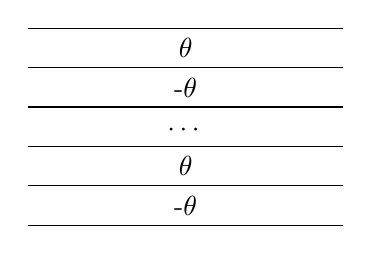
\begin{tikzpicture}
	\draw (0,0) -- (4,0);
	\draw (0,-0.5) -- (4,-0.5) node[midway, above] {$\theta$};
	\draw (0,-1) -- (4,-1) node[midway, above] {\text{-}$\theta$};
	\draw (0,-1.5) -- (4,-1.5) node[midway, above] {$\cdots$};
	\draw (0,-2) -- (4,-2) node[midway, above] {$\theta$};
	\draw (0,-2.5) -- (4,-2.5) node[midway, above] {\text{-}$\theta$};
\end{tikzpicture}
\caption{Model for Angle ply laminate}
\end{figure}


\section{Conclusion}
In this paper, SAGA is proposed to search the optimal lay-up for laminated composite under different
loading. Two situations are considered under the same loading, a set of two distinct angles, and
three distinct angles, SAGA can adjust its convergence speed depending on the difference of
individual's constraint value and constraint threshold.  








% conference papers do not normally have an appendix
% use section* for acknowledgement
\section*{Acknowledgment}


The authors would like to thank...


% trigger a \newpage just before the given reference
% number - used to balance the columns on the last page
% adjust value as needed - may need to be readjusted if
% the document is modified later
%\IEEEtriggeratref{8}
% The "triggered" command can be changed if desired:
%\IEEEtriggercmd{\enlargethispage{-5in}}

% references section

% can use a bibliography generated by BibTeX as a .bbl file
% BibTeX documentation can be easily obtained at:
% http://www.ctan.org/tex-archive/biblio/bibtex/contrib/doc/
% The IEEEtran BibTeX style support page is at:
% http://www.michaelshell.org/tex/ieeetran/bibtex/
%\bibliographystyle{IEEEtran}
% argument is your BibTeX string definitions and bibliography database(s)
%\bibliography{IEEEabrv,../bib/paper}
%
% <OR> manually copy in the resultant .bbl file
% set second argument of \begin to the number of references
% (used to reserve space for the reference number labels box)
%\begin{thebibliography}{1}

%\bibitem{IEEEhowto:kopka}
%H.~Kopka and P.~W. Daly, \emph{A Guide to \LaTeX}, 3rd~ed.\hskip 1em plus
%  0.5em minus 0.4em\relax Harlow, England: Addison-Wesley, 1999.

%\end{thebibliography}

\bibliographystyle{IEEEtran}
\bibliography{a5_reference}

\end{document}


